\documentclass[10pt,a4paper]{article}
\usepackage{xeCJK}
\usepackage[a4paper,left=20mm,right=20mm,top=25mm,bottom=20mm]{geometry}	%页边距
\usepackage{fancyhdr}	%页眉、页脚
\usepackage{indentfirst}	%首行缩进
\usepackage{graphicx}	%图片
\usepackage{textcomp}
\usepackage{subfigure}	
\usepackage{enumitem}
\usepackage{tabularx}
\usepackage{multirow}
\usepackage{caption}
\usepackage{amsmath}	%公式对齐
\usepackage{tikz-feynman}

\newcommand{\nexp}{霍尔效应}

%————页眉、页脚设置————
\thispagestyle{plain}
\pagestyle{fancy}
\fancyhf{}
\fancyhead[R]{PB22000195 王元叙}
\fancyhead[L]{\nexp}	%————————————
\fancyfoot[C]{\thepage}
\renewcommand{\headrulewidth}{0pt}
\renewcommand{\footrulewidth}{0pt}
%————————————

\setenumerate[1]{itemsep=0pt,partopsep=0pt,parsep=\parskip,topsep=5pt}
\setlength{\parindent}{2em}
\renewcommand\arraystretch{1.4}

\makeatletter
\newenvironment{figurehere}
{\def\@captype{figure}}
{}
\newenvironment{tablehere}
{\def\@captype{table}}
{}
\makeatother

\begin{document}
	%————起始————
	\vspace*{-5em}
	\begin{center}
		\includegraphics[width=0.6\textwidth]{Picture//USTC}\\
		\Large \textbf{大学物理-综合实验|实验报告}\\[5mm]

		\normalsize
		\begin{tabular}{ll}
			姓名 & \textbf{王元叙}\\
			学号 & \textbf{PB22000195}\\
			班级 & \textbf{22级少年班学院5班}\\
			日期 & \textbf{2023年5月22日}\\	
		\end{tabular}\\[5mm]

		\LARGE \textbf{\nexp}\\[5mm]	

	\end{center}
	%————————————

	%————正文————
	\section{实验目的}

	\begin{enumerate}
		\item 了解霍尔效应原理以及有关霍尔器件对材料要求的知识。
		\item 学习用“对称测量法”消除副效应影响。
		\item 根据霍尔电压判断霍尔元件载流子类型。
		\item 计算载流子的浓度和迁移速度。
	\end{enumerate}


	\section{实验装置}
	
	恒流源两个;电磁铁(4900Gs/A);霍尔样品和样品架;换向开关两只、导线若干;数字万用表一台;小磁针一只。



	\section{实验原理}

	\subsection{通过霍尔效应测量磁场}
	
	\begin{figurehere}
		\centering
		\includegraphics[width=0.95\linewidth]{pics/0.png}
		\caption*{\bf 图1.1 : 实验装置原理图及电磁铁气隙磁场}
	\end{figurehere}
	
	\subsection{霍尔效应实验中的副效应}

	在实际应用中, 伴随霍尔效应经常存在其他副效应。
	\begin{enumerate}
		\item {\bf 爱廷豪森效应} : 实际中载流子迁移速率 $u$ 服从 统计分布规律, 速度小的载流子受到的洛伦兹力小于霍尔电场作用力, 向霍尔电场作用力 方向偏转, 速度大的载流子受到磁场作用力大于霍尔电场作用力, 向洛伦兹力方向偏转。这 样使得一侧高速载流子较多, 相当于温度较高, 而另一侧低速载流子较多, 相当于温度较 低。这种横向温差就是温差电动势 $V_E$, 这种现象称为爱廷豪森效应。这种效应建立需要一 定时间, 如果采用直流电测量时会因此而给霍尔电压测量带来误差, 如果采用交流电, 则 由于交流变化快使得爱廷豪森效应来不及建立, 可以减小测量误差。
		\item {\bf 不等位效应} : 在使用霍尔元件时还存在不等位电动势引起的误差, 这是因为霍尔电极 $B, B^{\prime}$ 不可能绝对对称焊在霍尔片两侧产生的。由于目前生产工艺水平较高, 不等位电动势很小, 故一般可以忽略, 也可以用一个电位器加以平衡 (如图 1 中电位器 $R_1$ )。
		\item 此外其他副效应如能斯特效应、里纪-勒杜克效应等,可以使用用对称测量法消除。
		
	\end{enumerate}


	\subsection{堆成测量法的消除副效应}

	我们可以通过改变 $I_S$ 和磁场 $B$ 的方向消除大多数副效应,即堆成测量法。具体说在规定电流和磁场 正反方向后, 分别测量下列四组不同方向的 $I_S$ 和 $B$ 组合的 $V_{B B^{\prime}}$, 即
	$$
	\begin{array}{lll}
	+B, & +I & V_{B B^{\prime}}=V_1 \\
	-B, & +I & V_{B B^{\prime}}=-V_2 \\
	+B, & -I & V_{B B^{\prime}}=-V_3 \\
	-B, & -I & V_{B B^{\prime}}=V_4
	\end{array}
	$$

	然后得到霍尔电压平均值, 这样虽然不能消除所有的副效应, 但其引人的误差不大, 可以忽略不计。

	\subsection{电导率的测量方法}

	电导率测量原理如下图所示:
	
	\begin{figurehere}
		\centering
		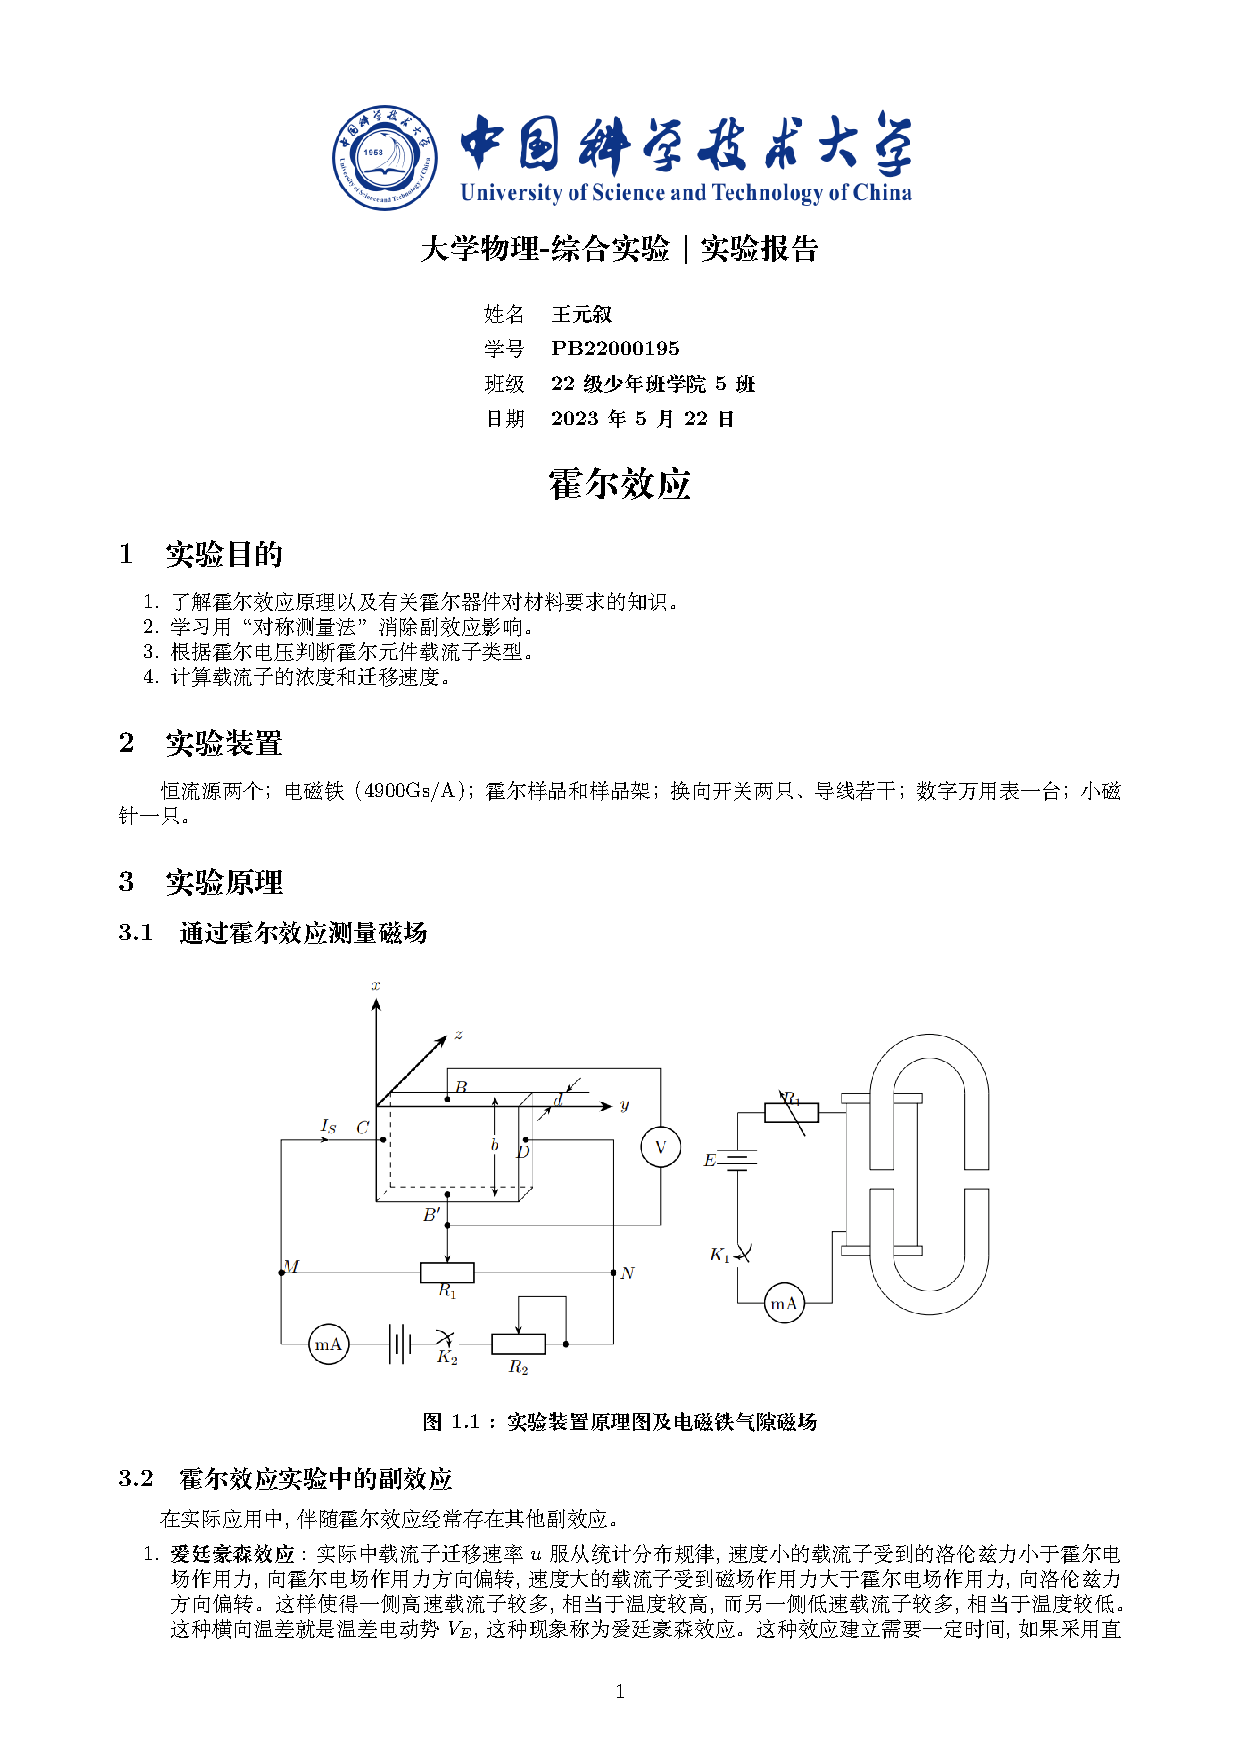
\includegraphics[width=0.45\linewidth]{pics/11.png}
		\caption*{\bf 图1.2 : 霍尔效应原理图}
	\end{figurehere}

	设 $B^{\prime}, A^{\prime}$ 间距离为 $L$, 样品横截面积为 $S=b d$, 流经样 品电流为 $I_S$, 在零磁场下, 测得 $B$ 间电压为 $V_{B^{\prime} A^{\prime}}$, 根据欧姆定律可以求出材料的电导率。 电导率 $\sigma$ 与载流子浓度 $n$ 及迁移率 $\mu$ 之间有如下关系:
	$$
	\sigma=n e \mu
	$$

	\section{实验步骤}
	
	\begin{enumerate}
		\item 用六脚霍尔片接好线路,霍尔片的尺寸为:d = 0.5mm, b = 4.0 mm,L= 3.0 mn

		\item 保持 $I_{M}$ 不变,取 $I_{M}=0.$ 45 A,$I_{S}$取$1.00, 1.50,\cdots,4.50$mA,测绘 $V_{H}-I_{S}$ 曲线,计算 $R_H$

		\item 保持 $I_{S}$ 不变,取Is = 4.50 mA,$I_{M}$取$0.100,0.150,\cdots,0.450$ A,测绘 $V_{H}-I_{M}$ 曲线,计算 $R_H$

		\item 在零磁场下,取 $I_{S}=1$ .00 mA,测$V_{B'A'}$

		\item 确定样品导电类型,并求 $R_H, n, \sigma, \mu$

		\item 使用四脚锑化铟片完成。取 $I_{S}$ = 1.00mA,Ix在0 - 0.800 A之间,测绘 $V_{H}-I_{M}$ 曲线
	\end{enumerate}
	
	\newpage
	\section{实验数据与分析}

	\subsection{保持励磁电流不变测量霍尔系数}

	保持励磁电流 $I_M = $

	\begin{tablehere}
		\caption*{\bf 表1 保持励磁电流不变测量霍尔系数数据}
		\noindent	
		\begin{center}
			\newcolumntype{Y}{>{\centering\arraybackslash}X}
			\begin{tabularx}{0.95\textwidth}{|Y|Y|Y|Y|Y|Y|}
				\hline
				1   & 2.87  & 2.79  & 2.83  & 2.84  & 2.81 \\ \hline
				1.5 & 4.05  & 4.05  & 4.11  & 4.11  & 4.08 \\ \hline
				2   & 5.35  & 5.36  & 5.44  & 5.44  & 5.40 \\ \hline
				2.5 & 6.77  & 6.75  & 6.67  & 6.66  & 6.61 \\ \hline
				3   & 8.09  & 8.09  & 7.97  & 7.95  & 8.05 \\ \hline
				3.5 & 9.43  & 9.41  & 9.27  & 9.27  & 9.39 \\ \hline
				4   & 10.75 & 10.75 & 10.58 & 10.57 & 10.67 \\ \hline
				4.5 & 12.09 & 12.08 & 11.89 & 11.88 & 11.99 \\ \hline
			\end{tabularx}
			\vspace*{1em}
		\end{center}
	\end{tablehere}

	其中第六列数据依据公式 $V_H = \frac{V_1 + V_2 + V_3 + V_4}{4}$ 计算得到。使用软件 Origin 拟合 $V_H - I_S$图线,如图所示: 

	\begin{figurehere}
		\centering
		\includegraphics[width=0.80\linewidth]{pics/1.png}
		\caption*{\bf 图2.1: $V_H − I_S$ 拟合图线}
	\end{figurehere}

	线性拟合斜率斜率 $k_1=2.634V/A, R^2=0.99999.$ ,经过计算可以得到:
	$$
	\begin{aligned}R_H&=\frac{V_H d}{I_S B}\\&=\frac{2.634V/A\times5\times10^{-4}m}{4900Gs/A\times0.45A\times10^{-4}T/Gs}\\&=5.97\times10^{-3}m^3/C\end{aligned}
	$$


	\newpage
	\subsection{保持样品电流不变测量霍尔系数}
	
	\begin{tablehere}
		\caption*{\bf 表2 保持样品电流不变测量霍尔系数数据}
		\noindent	
		\begin{center}
			\newcolumntype{Y}{>{\centering\arraybackslash}X}
			\begin{tabularx}{0.95\textwidth}{|Y|Y|Y|Y|Y|Y|}
				\hline
				0.1  & 2.72  & 2.72  & 2.53  & 2.53  & 2.63  \\ \hline
				0.15 & 4.02  & 4.05  & 3.89  & 3.90  & 3.97  \\ \hline
				0.2  & 5.34  & 5.38  & 5.20  & 5.21  & 5.28  \\ \hline
				0.25 & 6.66  & 6.69  & 6.51  & 6.50  & 6.59  \\ \hline
				0.3  & 8.00  & 8.02  & 7.84  & 7.84  & 7.93  \\ \hline
				0.35 & 9.33  & 9.36  & 9.17  & 9.18  & 9.26  \\ \hline
				0.4  & 10.75 & 10.70 & 10.52 & 10.51 & 10.62 \\ \hline
				0.45 & 12.08 & 12.08 & 11.89 & 11.90 & 11.99 \\ \hline
			\end{tabularx}
			\vspace*{1em}
		\end{center}
	\end{tablehere}

	其中第六列数据依据公式 $V_H = \frac{V_1 + V_2 + V_3 + V_4}{4}$ 计算得到。使用软件 Origin 拟合 $V_H - I_M$图线,如图所示: 

	\begin{figurehere}
		\centering
		\includegraphics[width=0.80\linewidth]{pics/2.png}
		\caption*{\bf 图2.2: $V_H − I_M$ 拟合图线}
	\end{figurehere}

	线性拟合斜率 $k_{2}=26.686mV/A,R^{2}=0.999$ ,计算可得:
	$$
	\begin{aligned}R_H&=\frac{V_H d}{I_S B}\\&=\frac{26.686 \times 10 ^ {-3}V/A\times5\times10^{-4}m}{4900Gs/A\times0.0045A\times10^{-4}T/Gs}\\&=6.05\times10^{-3}m^3/C\end{aligned}
	$$
	
	
	\newpage
	\subsection{零磁场下测量横向电势差}
	
	零磁场下, $I_S=1 \mathrm{~mA}$, 测得 $V_{x x}=67.10 \mathrm{mV}$ 。在上面两个实验中我们使用不同方法测得了两个 $R_H$ 值,在下面的计算中我们使用二者的平均值
	$$
	R_h = \frac{6.05 + 5.97}{2}\times 10 ^ {-3}m^3/C = 6.01 \times 10 ^ {-3}m^3 /C
	$$

	于是我们可以计算得到:
	$$
	\begin{aligned}
	\sigma & =\frac{1}{\rho} \\
	& =\frac{L}{b d} \frac{I_S}{V_{x x}} \\
	& =\frac{3}{4 \times 0.5 \times 67.10 \times 10^{-3}} \\
	& =22.355 \mathrm{~S} / \mathrm{m} \\
	n & =\frac{1}{R_H q} \\
	& =\frac{1}{6.01 \times 10^{-3} \cdot 1.60 \times 10^{-19}} \\
	& =1.04 \times 10^{21} \\
	\mu & =\frac{\sigma}{n q} \\
	& =\frac{22.355}{1.04 \times 10^{21} \cdot 1.6 \times 10^{-19}} \\
	& =0.134 \mathrm{~m}^2 / \mathrm{V} \cdot \mathrm{s}
	\end{aligned}
	$$

	\subsection{确定样品导电类型}

	使用小磁针放在电磁铁的正上方,根据小磁针方向指向南方可以分析:
	
	\begin{figurehere}
		\centering
		\includegraphics[width=0.80\linewidth]{pics/4.png}
		\caption*{\bf 图3: 导电类型分析图}
	\end{figurehere}

	可以知道载流子是n型。

	\newpage
	\subsection{使用锑化铟片绘制 $V_H − I_M$ 图像}

	保持样品电流 $I_S = 1\text{mA}$不变
	\begin{tablehere}
		\caption*{\bf 表3 锑化铟片测量原始数据}
		\noindent	
		\begin{center}
			\newcolumntype{Y}{>{\centering\arraybackslash}X}
			\begin{tabularx}{0.45\textwidth}{|Y|Y|Y|Y|}
				\hline
				0.040 & 46.85  &
				0.080 & 91.14  \\ \hline
				0.120 & 133.52 &
				0.160 & 172.41 \\ \hline
				0.200 & 201.70 &
				0.240 & 219.32 \\ \hline
				0.280 & 233.56 &
				0.320 & 245.73 \\ \hline
				0.360 & 257.08 &
				0.400 & 268.53 \\ \hline
				0.440 & 280.49 &
				0.480 & 293.54 \\ \hline
				0.520 & 304.83 &
				0.560 & 316.75 \\ \hline
				0.600 & 328.54 &
				0.640 & 340.57 \\ \hline
				0.680 & 352.72 &
				0.720 & 364.32 \\ \hline
				0.760 & 375.89 &
				0.800 & 387.60 \\ \hline
			\end{tabularx}
			\vspace*{1em}
		\end{center}
	\end{tablehere}

	使用软件绘图可以得到:

	\begin{figurehere}
		\centering
		\includegraphics[width=0.80\linewidth]{pics/3.png}
		\caption*{\bf 图4: 锑化铟片 $V_H − I_M$ 拟合图线}
	\end{figurehere}

	可以观察到在某个拐点以后曲线的斜率发生了突变。

\end{document}